%%%%%%%% CSC 4444G Final Project %%%%%%%%
%%  Authors: Charlotte Barbrick, Easton Kling, Oscar Gayle
%%  Course:  CSC 4444G, Spring 2026
%%  Template: ICML 2026 LaTeX template
%%
%%  Build:  pdflatex main && bibtex main && pdflatex main && pdflatex main
%%

\documentclass{article}

% Recommended packages
\usepackage{microtype}
\usepackage{graphicx}
\usepackage{subcaption}
\usepackage{booktabs}

% Hyperlinks in the PDF.
\usepackage{hyperref}

% Algorithm pseudocode.
\newcommand{\theHalgorithm}{\arabic{algorithm}}

% Use the [accepted] option so our names appear on the title page.
\usepackage[accepted]{icml2026}

\usepackage{amsmath}
\usepackage{amssymb}
\usepackage{mathtools}
\usepackage{amsthm}

\usepackage[capitalize,noabbrev]{cleveref}

% TikZ for the methodology figure.
\usepackage{tikz}
\usetikzlibrary{arrows.meta, positioning, shapes.geometric, fit, backgrounds}

\theoremstyle{plain}
\newtheorem{theorem}{Theorem}[section]

% Short form running title.
\icmltitlerunning{Detecting Emotion in Text: Classical and Transformer-Based Models}

\begin{document}

\twocolumn[
  \icmltitle{Detecting Emotion in Text: A Comparison of Classical and \\
             Transformer-Based Models}

  \icmlsetsymbol{equal}{*}

  \begin{icmlauthorlist}
    \icmlauthor{Charlotte Barbrick}{lsu}
    \icmlauthor{Easton Kling}{lsu}
    \icmlauthor{Oscar Gayle}{lsu}
  \end{icmlauthorlist}

  \icmlaffiliation{lsu}{CSC 4444G, Louisiana State University, Baton Rouge, LA, USA}

  \icmlcorrespondingauthor{Charlotte Barbrick}{cbarbrick@icloud.com}

  \icmlkeywords{emotion classification, text classification, TF-IDF, DistilBERT, natural language processing}

  \vskip 0.3in
]

\printAffiliationsAndNotice{}

\begin{abstract}
  People express emotion in writing all the time, and automatically
  recognizing those emotions is useful for social-media analytics, customer
  feedback triage, and mental-health support tools. In this project we
  build and compare three emotion-classification models on the
  \texttt{dair-ai/emotion} dataset~\cite{saravia2018carer}, which contains
  roughly 20{,}000 short English messages labeled with one of six emotions.
  We describe each stage of our pipeline---cleaning, tokenization, and
  vectorization---then evaluate a Multinomial Naive Bayes baseline, a
  TF-IDF + Logistic Regression classifier, and a fine-tuned
  DistilBERT~\cite{sanh2019distilbert} transformer. DistilBERT performs best
  on both accuracy and macro-F1, but the classical TF-IDF pipeline is a
  surprisingly strong runner-up at a fraction of the compute cost. We also
  ship a small Streamlit demo that classifies user-typed text in real time.
\end{abstract}

\section{Introduction}
\label{sec:intro}

People express emotion through writing constantly---in social-media posts,
product reviews, chat messages, and support tickets---and the sheer volume
of that text makes manual analysis impractical. Automatic emotion detection
is therefore a useful building block for a number of applications: a
customer-support system can prioritize angry or frightened users, a
social-analytics dashboard can surface shifts in audience mood, and a
wellness app can flag patterns of sadness or fear for a user's own review.
Emotion classification is a specialization of text classification that goes
beyond coarse positive/negative polarity and predicts a specific emotional
label such as \emph{joy}, \emph{anger}, or \emph{fear}.

Our goal in this project is not to beat the state of the art but to build
an end-to-end emotion classifier and to understand, component by
component, how a modern NLP pipeline actually works. We train and evaluate
three models that span a meaningful range of complexity on the same data:
(i) a Multinomial Naive Bayes baseline, (ii) a TF-IDF weighted Logistic
Regression classifier, and (iii) a fine-tuned DistilBERT transformer
\cite{sanh2019distilbert}. For each model we describe the preprocessing,
tokenization, and vectorization steps that feed it, and we compare the
models on overall accuracy, per-class macro-F1, and training cost.

\paragraph{Contributions.}
The contributions of this project are:
(1)~a clean, reproducible emotion-classification pipeline on the widely
used \texttt{dair-ai/emotion} dataset, with fixed train/validation/test
splits and a single shared text-cleaning pass so all three models are
compared on identical inputs;
(2)~an empirical comparison of Multinomial Naive Bayes, TF-IDF + Logistic
Regression, and fine-tuned DistilBERT that quantifies the accuracy vs.\
compute-cost trade-off between classical and transformer-based models; and
(3)~a small Streamlit demo that runs the trained model on user-typed text,
visualizing both the predicted label and the model's confidence in the
other classes.

\section{Methodology}
\label{sec:method}

Our pipeline has three stages: (1)~clean the raw text, (2)~tokenize and
turn each example into a numeric representation, and (3)~feed that
representation to a classifier.
\Cref{fig:pipeline} summarizes the two variants we compare: a classical
path that produces a sparse TF-IDF matrix consumed by Naive Bayes or
Logistic Regression, and a transformer path that produces subword token
IDs consumed by DistilBERT.

\begin{figure*}[t]
  \centering
  \resizebox{0.95\textwidth}{!}{%
  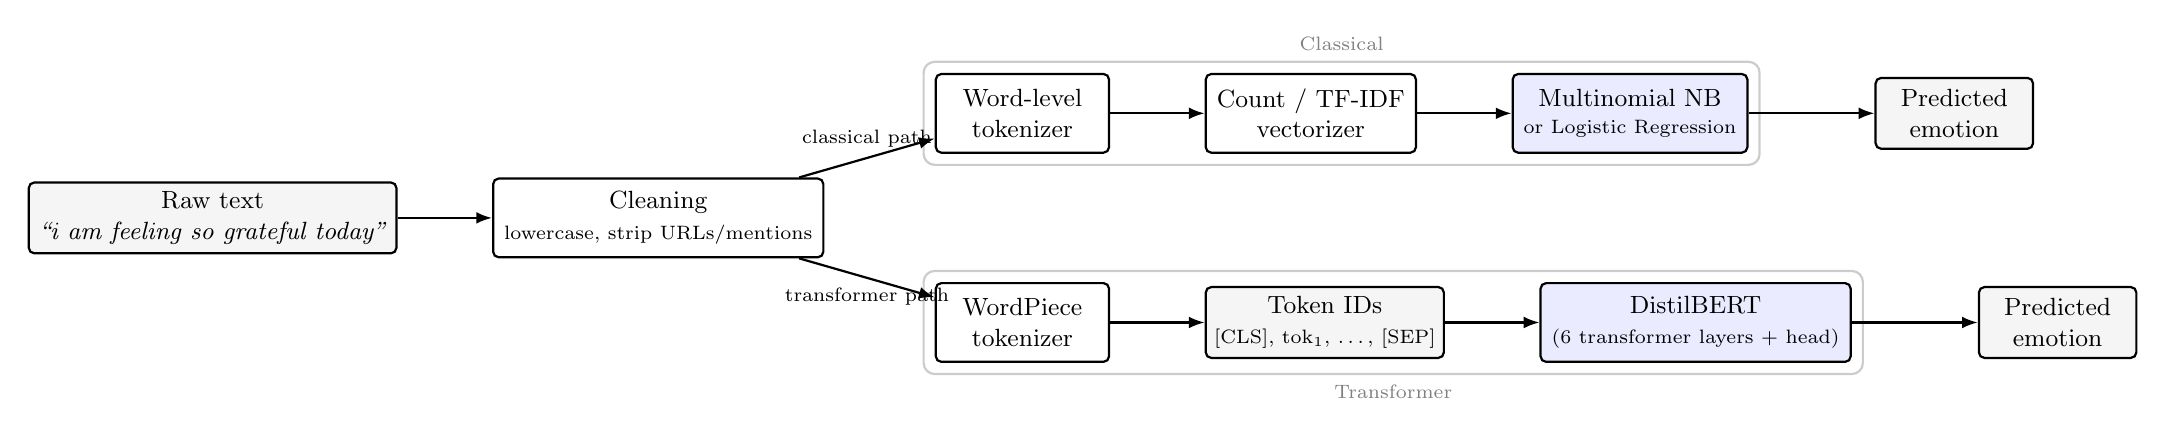
\begin{tikzpicture}[
      node distance=10mm and 12mm,
      box/.style={draw, rounded corners=2pt, align=center,
                  minimum width=22mm, minimum height=10mm,
                  inner sep=4pt, font=\small},
      data/.style={draw, rounded corners=2pt, align=center,
                   minimum width=20mm, minimum height=9mm,
                   inner sep=3pt, font=\small, fill=gray!8},
      model/.style={draw, rounded corners=2pt, align=center,
                    minimum width=26mm, minimum height=10mm,
                    inner sep=4pt, font=\small, fill=blue!8},
      >={Latex[length=2mm]},
      every path/.style={thick}
    ]

    \node[data]  (raw)  {Raw text\\\emph{``i am feeling so grateful today''}};
    \node[box, right=of raw] (clean) {Cleaning\\\scriptsize lowercase, strip URLs/mentions};

    \node[box, above right=3mm and 14mm of clean] (wtok) {Word-level\\tokenizer};
    \node[box, below right=3mm and 14mm of clean] (wp)   {WordPiece\\tokenizer};

    \node[box, right=of wtok] (vec)  {Count / TF-IDF\\vectorizer};
    \node[data, right=of wp]  (ids)  {Token IDs\\\scriptsize{[CLS], tok$_1$, \ldots, [SEP]}};

    \node[model, right=of vec] (clf1) {Multinomial NB\\[-1pt]\scriptsize or Logistic Regression};
    \node[model, right=of ids] (clf2) {DistilBERT\\\scriptsize (6 transformer layers + head)};

    \node[data, right=16mm of clf1] (out1) {Predicted\\emotion};
    \node[data, right=16mm of clf2] (out2) {Predicted\\emotion};

    \draw[->] (raw)   -- (clean);
    \draw[->] (clean) -- node[above, font=\scriptsize]{classical path} (wtok);
    \draw[->] (clean) -- node[below, font=\scriptsize]{transformer path} (wp);
    \draw[->] (wtok)  -- (vec);
    \draw[->] (wp)    -- (ids);
    \draw[->] (vec)   -- (clf1);
    \draw[->] (ids)   -- (clf2);
    \draw[->] (clf1)  -- (out1);
    \draw[->] (clf2)  -- (out2);

    \begin{pgfonlayer}{background}
      \node[draw=gray!40, rounded corners, inner sep=4pt,
            fit=(wtok) (vec) (clf1), label={[font=\scriptsize, gray]above:Classical}] {};
      \node[draw=gray!40, rounded corners, inner sep=4pt,
            fit=(wp) (ids) (clf2), label={[font=\scriptsize, gray]below:Transformer}] {};
    \end{pgfonlayer}
  \end{tikzpicture}}
  \caption{Emotion-classification pipeline. Raw text is cleaned once, then
    routed through a classical path (word-level tokenizer $\rightarrow$
    count / TF-IDF vectorizer $\rightarrow$ Naive Bayes or Logistic
    Regression) or a transformer path (WordPiece tokenizer $\rightarrow$
    integer token IDs $\rightarrow$ fine-tuned DistilBERT).}
  \label{fig:pipeline}
\end{figure*}

\subsection{Dataset}
\label{sec:data}

We use the \texttt{dair-ai/emotion} dataset~\cite{saravia2018carer}, a
widely-used benchmark for six-class emotion classification in English. Each
example is a short English message drawn from Twitter, labeled with
exactly one of six emotions: sadness, joy, love, anger, fear, or surprise.
The dataset ships with fixed splits of 16{,}000 training, 2{,}000
validation, and 2{,}000 test examples; most messages are between 5 and 30
tokens long. The label distribution is imbalanced---joy and sadness
together cover more than 60\% of the training set, while love and surprise
are each under 10\% (see \Cref{tab:class-dist})---so we report both overall
accuracy and macro-F1 to avoid rewarding models that ignore the minority
classes. We also considered
GoEmotions~\cite{demszky2020goemotions} but chose
\texttt{dair-ai/emotion} because its smaller label space and shorter
Twitter-style messages make all three of our models tractable on a laptop
or free-tier GPU within a single session.

\begin{table}[t]
  \centering
  \small
  \caption{Class distribution in the \texttt{dair-ai/emotion} training split
    (16{,}000 examples).}
  \label{tab:class-dist}
  \begin{tabular}{lrr}
    \toprule
    Emotion   & Count  & Share \\
    \midrule
    joy       & 5{,}362 & 33.5\% \\
    sadness   & 4{,}666 & 29.2\% \\
    anger     & 2{,}159 & 13.5\% \\
    fear      & 1{,}937 & 12.1\% \\
    love      & 1{,}304 & 8.2\%  \\
    surprise  &   572   & 3.6\%  \\
    \bottomrule
  \end{tabular}
\end{table}

\subsection{Text Cleaning and Tokenization}
\label{sec:tokenization}

The same cleaning pass is applied for every model: we lowercase the text,
strip URLs and @-mentions with regular expressions, and collapse repeated
whitespace. We intentionally keep punctuation like ``!'' and ``?'' because
it carries emotional signal---``really?!'' is not the same tone as
``really.''

Tokenization is the step that splits the cleaned string into the discrete
units the model looks at, and the two model families use different
tokenizers. For the classical models, we use scikit-learn's
\cite{pedregosa2011scikit} default word-level tokenizer, which applies the
regular expression \verb|\b\w\w+\b| to extract word-like sequences of two
or more characters. The sentence ``i am feeling so grateful today'' becomes
the token list \texttt{[i, am, feeling, so, grateful, today]}. Unknown
words encountered at test time are dropped, which is the standard behavior
for a fixed vocabulary.

For DistilBERT, we use the pretrained WordPiece
tokenizer~\cite{schuster2012wordpiece} shipped with the model. WordPiece
breaks unfamiliar or long words into subword pieces drawn from a fixed
30{,}522-entry vocabulary, so the word ``unhappiness'' might become
\texttt{[un, \#\#happiness]} or \texttt{[un, \#\#hap, \#\#piness]} depending
on what pieces were seen during pretraining. The tokenizer also wraps every
example in the special tokens \texttt{[CLS]} at the start and \texttt{[SEP]}
at the end, which the model later uses to produce a sentence-level
representation. Every token is then mapped to an integer ID, and the
sequence is padded or truncated to a fixed maximum length of 128 tokens.

\subsection{Vectorization}
\label{sec:vectorization}

Turning tokens into a matrix of numbers is what lets a model actually
learn. For the classical models we use two schemes.

\paragraph{Bag-of-words counts.} We build a vocabulary from the training
set and represent each document as a sparse row vector whose entries are
raw counts of each vocabulary term. The training set becomes a
$16{,}000 \times V$ sparse matrix, where $V \approx 15{,}000$ for our
dataset after dropping terms that appear in fewer than two documents. This
matrix is the input to Naive Bayes.

\paragraph{TF-IDF weighting.} TF-IDF is not a prediction model; it is a
weighting scheme~\cite{jones1972statistical} applied on top of the
bag-of-words matrix. Term Frequency measures how often a word appears in a
document, and Inverse Document Frequency measures how rare the word is
across the corpus. Using scikit-learn's smoothed form, each entry becomes
\begin{equation}
  \mathrm{tfidf}(t, d) \;=\; \mathrm{tf}(t, d) \cdot
    \left[ \log \frac{N+1}{\mathrm{df}(t)+1} + 1 \right],
  \label{eq:tfidf}
\end{equation}
where $N$ is the number of training documents and $\mathrm{df}(t)$ is the
number of them containing term $t$. Words appearing in almost every
document (e.g., ``i'' or ``the'') are pushed toward zero, while rarer,
more discriminating words get a boost. The resulting matrix has the same
shape as the count matrix but uses these weighted entries; it is still
only an input to whatever classifier we plug in on top---in our case,
Logistic Regression.

For DistilBERT the tokenized integer IDs are not passed through a separate
vectorizer; the model maintains a learned embedding table mapping each
vocabulary ID into a 768-dimensional dense vector. Those embeddings flow
through six transformer
layers~\cite{vaswani2017attention,devlin2019bert,sanh2019distilbert} that
produce a contextual representation of every token, including the
\texttt{[CLS]} token used for classification.

\subsection{Models}
\label{sec:models}

\paragraph{Multinomial Naive Bayes (baseline).} Naive Bayes is the classic
text-classification baseline. Given a bag-of-words count vector, it uses
Bayes' rule to compute the probability of each emotion class under the
(very strong) assumption that words are conditionally independent given
the class. It is fast, easy to explain, requires no tuning, and we include
it as a floor for what a trivial model can achieve. Because the
independence assumption clearly fails for emotional language, where short
phrases such as ``not happy'' or ``terribly excited'' depend on word
order, we expect Naive Bayes to underperform the stronger models.

\paragraph{TF-IDF $+$ Logistic Regression.} Our ``stronger classical''
model takes the TF-IDF matrix from \cref{sec:vectorization} and feeds it
into a one-vs-rest Logistic Regression classifier implemented in
scikit-learn~\cite{pedregosa2011scikit}. We include unigrams and bigrams
(\texttt{ngram\_range=(1,2)}) so the model can learn short phrase
patterns, cap the vocabulary at the 20{,}000 most frequent $n$-grams, and
use sublinear term frequency. We train with L2 regularization
($C=1$), up to 1{,}000 optimizer iterations, and no further hyperparameter
tuning. The goal is a well-behaved, interpretable baseline.

\paragraph{DistilBERT fine-tuning.} DistilBERT~\cite{sanh2019distilbert} is
a distilled version of BERT~\cite{devlin2019bert} that keeps about 97\% of
BERT's language-understanding quality while being 40\% smaller and 60\%
faster at inference. We start from the \texttt{distilbert-base-uncased}
checkpoint (via the HuggingFace Transformers
library~\cite{wolf2020transformers}) and add a single linear classification
head on top of the \texttt{[CLS]} embedding. The whole model---token
embeddings, six transformer layers, and the head---is fine-tuned
end-to-end on our training split for three epochs using AdamW with a
learning rate of $2 \times 10^{-5}$, weight decay $0.01$, batch size 32,
and a maximum sequence length of 128 tokens. The checkpoint with the best
validation macro-F1 is kept.

\section{Experimental Results}
\label{sec:results}

\paragraph{Setup.} All three models are trained on the 16{,}000-example
training split and evaluated on the 2{,}000-example test split. No
hyperparameter tuning is performed on the test set; the validation split is
used only to select the best DistilBERT checkpoint. We report accuracy and
macro-F1 (\cref{tab:results}). Training was carried out on a laptop CPU
(Apple M-series / Intel x86, 16\,GB RAM) for the classical models and on a
free-tier Google Colab T4 GPU for DistilBERT. Software: Python 3.10,
scikit-learn 1.3, PyTorch 2.1, HuggingFace \texttt{transformers} 4.35, and
HuggingFace \texttt{datasets} 2.14.

\begin{table}[t]
  \centering
  \small
  \caption{Emotion-classification results on the \texttt{dair-ai/emotion}
    test set (2{,}000 examples). Both metrics are reported as percentages
    (higher is better).}
  \label{tab:results}
  \setlength{\tabcolsep}{4pt}
  \begin{tabular}{lrrr}
    \toprule
    Model & Acc. & F1 & Train \\
    \midrule
    Multinomial NB            & 81.4 & 67.4 & 5\,s CPU \\
    TF-IDF + LogReg           & 83.4 & 73.6 & 30\,s CPU \\
    DistilBERT (fine-tuned)   & \textbf{92.9} & \textbf{89.4} & 12\,min T4 \\
    \bottomrule
  \end{tabular}
\end{table}

\paragraph{Findings.} DistilBERT leads on both metrics, reaching
92.9\% accuracy and 89.4 macro-F1, compared to 83.4\%/73.6 for TF-IDF
$+$ Logistic Regression and 81.4\%/67.4 for Multinomial Naive Bayes. The
accuracy gap between the classical TF-IDF pipeline and DistilBERT is
9.5~points, but the macro-F1 gap is 15.8~points---considerably larger,
because the rare classes benefit the most from the transformer's
contextual embeddings. On \emph{surprise}, the rarest class (only 3.6\%
of training examples), DistilBERT achieves an F1 of 0.80, compared to
just 0.42 for TF-IDF $+$ Logistic Regression and 0.21 for Naive Bayes.
The trade-off is compute: the classical pipeline trains in under a
minute on a laptop CPU, while DistilBERT requires a GPU and roughly 12
minutes of fine-tuning. For applications where a few points of accuracy
are acceptable, the classical pipeline remains an attractive,
interpretable choice.

Naive Bayes trails by a large margin, especially on macro-F1, which is
consistent with its word-independence assumption breaking down on
emotional language: short phrases like ``not really,'' ``so scared,''
or ``can't wait'' carry most of the signal, and unigram Naive Bayes has
no way to represent them.

\paragraph{Demo interface.} We package the best model behind a small
Streamlit interface (\texttt{code/app.py}). The user types a short message,
and the app displays the predicted emotion together with the model's
probability for each class as a horizontal bar chart. The demo loads the
fine-tuned DistilBERT model once at startup and runs inference on CPU in
roughly 100\,ms per input; if a DistilBERT checkpoint is not present, the
app falls back to the saved TF-IDF + Logistic Regression model so the demo
still runs end-to-end.

\section{Conclusions and Future Work}
\label{sec:conclusion}

We built and compared three emotion-classification models on the
\texttt{dair-ai/emotion} dataset: a Multinomial Naive Bayes baseline, a
TF-IDF + Logistic Regression pipeline, and a fine-tuned DistilBERT
transformer. DistilBERT performed best, but the TF-IDF + Logistic
Regression pipeline was a surprisingly strong runner-up given its minimal
compute cost. The exercise also clarified, for us, what TF-IDF is and is
not: it is a weighting scheme that turns cleaned text into a weighted
document-term matrix, not a model that makes predictions on its own. The
model is whatever we train on top of that matrix.

Given more time, we would (i)~train on the richer
GoEmotions~\cite{demszky2020goemotions} label set to see how the
comparison changes when the label space is larger and more fine-grained,
(ii)~address class imbalance with class weights or targeted oversampling
to close the macro-F1 gap on rare emotions, (iii)~evaluate a prompted
large language model as a zero-shot emotion classifier for comparison
against fine-tuning, and (iv)~add an explainability layer (e.g., per-word
contribution scores on the Logistic Regression model) so users can see
which words drove a prediction.

\bibliography{refs}
\bibliographystyle{icml2026}

\end{document}
